\chapter{Advanced Biological Computing in Python}
\label{chap:pythonII}

\epigraph{...some things in life are bad. They can really make you mad. 
Other things just make you swear and curse. When you're chewing on 
life's gristle, don't grumble; give a whistle, and this'll help things 
turn out for the  best. And... always look on the bright side of 
life...}{\textit{---Guess who?}}

In this chapter, we will cover a some topics in Python that will 
round-off your python training:
\begin{itemize}
	\item Numerical computing in python 
	\item ``Reading'' text data using regular expressions in python
	\item Databases, and using python to build and manage them
	\item Using python to build workflows
	% \item Interactive analysis and visualization of mathematical models as well as data using jupyter notebooks
\end{itemize}  
{\it The last topic will be necessary for your Miniproject, which will 
involve building a reproducible computational workflow.  }

\section{Numerical computing in {\tt python}}

The python package {\tt scipy} can help you do serious number crunching 
including,
	\begin{compactitem}
		\item Linear algebra (matrix and vector operations)
		\item Numerical integration (Solving ODEs)
		\item Fourier transforms
		\item Interpolation
		\item Calculating special functions (incomplete Gamma, Bessel, etc.)
		\item Generation of random numbers
		\item Using statistical functions and transformations
	\end{compactitem}
	
In the following, we will use the {\tt array} data structure in {\tt 
scipy} for data manipulations and calculations. Scipy arrays are 
objects, and are similar in some respects to python lists, but are more 
naturally multidimensional, homogeneous in type (the default is float), 
and allow efficient (fast) manipulations. Thus scipy arrays are 
analogous to the R {\tt matrix} data object/structure. 

\begin{tipbox}
	The same array objects are accessible within the {\tt numpy} package, which 
is a subset of {\tt scipy}.
\end{tipbox}

So let's try {\tt scipy}:
 \begin{lstlisting}
In []: import scipy

In []: a = scipy.array(range(5)) # a one-dimensional array

In []: a
Out[]: array([0, 1, 2, 3, 4])

In []: type(a)
Out[]: numpy.ndarray

In []: type(a[0])
Out []: numpy.int64
\end{lstlisting}

So all elements in {\tt a} are of type {\tt int} because that is what 
{\tt range()} returns (try {\tt ?range}).

\begin{figure}[H] \centering
    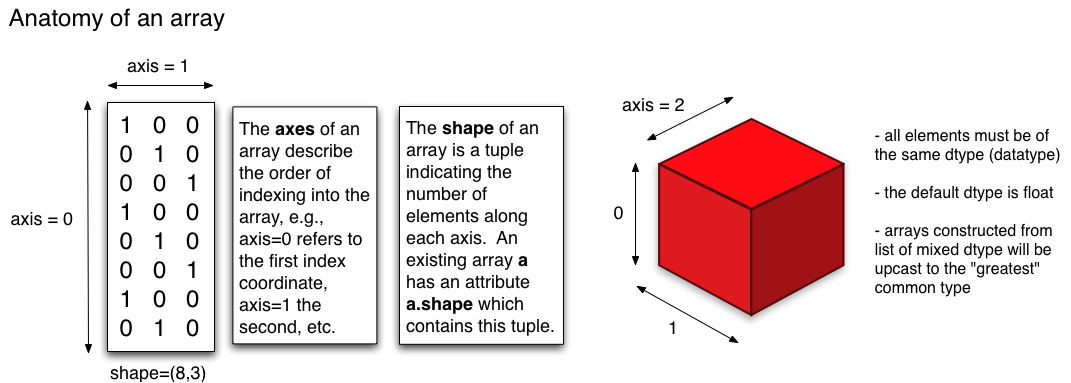
\includegraphics[width=1\textwidth]{numpyarray.png}
	\caption{A graphical depiction of numpy/scipy arrays, which can have 
	multiple dimensions (even greater than 3). From 
	\url{http://pages.physics.cornell.edu/~myers/teaching/ComputationalMethods/python/arrays.html}}
\end{figure}

You can also specify the data type of the array:

\begin{lstlisting}
In []: a = scipy.array(range(5), float)

In []: a
Out[]: array([ 0.,  1.,  2.,  3.,  4.])

In []: a.dtype # Check type 
Out[]: dtype('float64')
\end{lstlisting}

You can also get a 1-D arrays as follows: 
\begin{lstlisting}
In []: x = scipy.arange(5)

In []: x
Out[8]: array([0, 1, 2, 3, 4])

In [9]: x = scipy.arange(5.) #directly specify float using decimal

In [10]: x
Out[10]: array([ 0.,  1.,  2.,  3.,  4.])
\end{lstlisting}

As with other Python variables (e.g., created as a list or a 
dictionary), you can apply methods to variables created as scipy 
arrays. For example, TAB after {\tt x.} to see methods you can apply to 
{\tt x}:
\begin{lstlisting}
In [11]: x. 
x.T             x.conj          x.fill          
x.nbytes        x.round         x.take
x.all           x.conjugate     x.flags         
x.ndim          x.searchsorted  x.tofile
x.any           x.copy          x.flat          
x.newbyteorder  x.setfield      x.tolist
x.argmax        x.ctypes        x.flatten       
x.nonzero       x.setflags      x.tostring
x.argmin        x.cumprod       x.getfield      
x.prod          x.shape         x.trace
x.argsort       x.cumsum        x.imag         
x.ptp           x.size          x.transpose
x.astype        x.data          x.item          
x.put           x.sort          x.var
x.base          x.diagonal      x.itemset       
x.ravel         x.squeeze       x.view
x.byteswap      x.dot           x.itemsize      
x.real          x.std           
x.choose        x.dtype         x.max           
x.repeat        x.strides       
x.clip          x.dump          x.mean          
x.reshape       x.sum           
x.compress      x.dumps         x.min           
x.resize        x.swapaxes      

In [12]: x.shape
Out[12]: (5,)
\end{lstlisting}

\begin{tipbox}
	Remember, you can type {\tt :?x.methodname} to get info on a particular method. For 
example, try {\tt ?x.shape}.
\end{tipbox}

You can also convert to and from Python lists:

\begin{lstlisting}
In []: b = scipy.array([i for i in range(100) if i%2==1]) #odd numbers 
between 1 and 100

In []: c = b.tolist() #convert back to list
 \end{lstlisting}

To make a  matrix, you need a 2-D scipy array:
\begin{lstlisting}
In [14]: mat = scipy.array([[0, 1], [2, 3]])

In []: mat.shape
Out[]: (2, 2)
\end{lstlisting}

\subsection{Indexing and accessing arrays}

As with other Python data objects such as lists, scipy array elements 
can be accessed using square brackets ([]) with the [row,column] 
reference. Indexing of scipy arrays works 
like that for other data strauctures, with index values starting at 0. 
So, you can obtain all the elements of a particular row as:
\begin{lstlisting}
In []: mat[1] # accessing whole 2nd row, remember indexing starts at 
0
Out[]: array([2, 3])

In [57]: mat[:,1] #accessing whole second column  
Out[57]: array([1, 3])
\end{lstlisting}

And accessing particular elements: 
\begin{lstlisting}
In []: mat[0,0] # 1st row, 1st column element
Out[]: 0
In []: mat[1,0] # 2nd row, 1st column element
Out[]: 2
\end{lstlisting}
Note that (like all other programming languages) row index always comes 
before column index. That is, {\tt mat[1]} is always going to mean 
``whole second row'', and {\tt mat[1,1]} means 1st row and 1st column 
element. Therefore, to access the whole second column, you need:
\begin{lstlisting}
In []: mat[:,0] #accessing whole first column  
Out[]: array([0, 2])
\end{lstlisting}

\begin{tipbox}
Python indexing also accepts negative values for going back to the 
start from the end of an array:
\begin{lstlisting}
In []: mat[0,1]
Out[]: 1

In []: mat[0,-1] #interesting!
Out[]: 1

In []: mat[0,-2] #very interesting, perhaps useless!
Out[]: 0
\end{lstlisting}
\end{tipbox}

\subsection{Manipulating arrays}
Manipulating {\tt scipy} arrays is pretty straightforward.
 
 
\begin{tipbox}
A NumPy array is basically described by metadata (number of dimensions, shape, data type, and so on) and the actual data. The data is stored in a homogeneous and contiguous block of memory, at a particular address in system memory (Random Access Memory, or RAM). This block of memory is called the data buffer. This is the main difference with a pure Python structure, like a list, where the items are scattered across the system memory. This aspect is the critical feature that makes NumPy arrays so efficient.
\end{tipbox}

\subsubsection{Replacing, adding or deleting elements} 

Let's look at how you can replace, add, or delete an array element (a 
single entry, or whole row(s) or whole column(s)):

\begin{lstlisting}
In []: mat[0,0] = -1 #replace a single element

In []: mat
Out[]: 
array([[-1,  1],
       [ 2,  3]])
       
In []: mat[:,0] = [12,12] #replace whole column

In []: mat
Out[]: 
array([[12,  1],
       [12,  3]])

In []: scipy.append(mat, [[12,12]], axis = 0) #append row, note axis 
specification
Out[]: 
array([[12,  1],
       [12,  3],
       [12, 12]])

In []: scipy.append(mat, [[12],[12]], axis = 1) #append column
Out[]: 
array([[12,  1, 12],
       [12,  3, 12]])

In []: newRow = [[12,12]] #create existing row

In []: mat = scipy.append(mat, newRow, axis = 0) #append that existing row
Out[]: 
array([[12,  1],
       [12,  3],
       [12, 12]])

In []: scipy.delete(mat, 2, 0) #Delete 3rd row
Out[]: 
array([[12,  1],
       [12,  3]])
\end{lstlisting}

And concatenation:

\begin{lstlisting}
In []: mat = scipy.array([[0, 1], [2, 3]])

In []: mat0 = scipy.array([[0, 10], [-1, 3]])

In []: scipy.concatenate((mat, mat0), axis = 0)
Out[]: 
array([[ 0,  1],
       [ 2,  3],
       [ 0, 10],
       [-1,  3]])
\end{lstlisting}
 
\subsubsection{Flattening or reshaping arrays} 
You can also ``flatten'' or ``melt'' arrays, that is, change array 
dimensions (e.g., from a matrix to a vector):
\begin{lstlisting}
In []: mat.ravel()
Out[]: array([0, 1, 2, 3]) # NOTE: ravel is row-priority

In []: mat.reshape((4,1)) # this is different from ravel - check ?scipy.reshape
Out[66]: 
array([[0],
       [1],
       [2],
       [3]])

In []: mat.reshape((1,4)) # NOTE: reshaping is also row-priority
Out[]: array([[0, 1, 2, 3]])

In []: mat.reshape((3, 1)) # But total elements must remain the same!
---------------------------------------------------------------------------
ValueError                                Traceback (most recent call last)
<ipython-input-81-ba16cb0744eb> in <module>()
----> 1 mat.reshape((3, 1))

ValueError: total size of new array must be unchanged
\end{lstlisting}
This is a bit different than how {\tt R} behaves (coming up in Chapters 
(\ref{chap:RI}--\ref{chap:R_II} )), where you won't get an error ({\tt 
R} ``recycles'' data), which is more dangerous!

\subsection{Pre-allocating arrays}
As in other computer languages, it is usually more efficient to 
preallocate a array rather than append / insert / concatenate addtional 
elelents, rows, or columns. For example, if you know the size of your 
matrix or array, you can inititalize it with ones or zeros:

\begin{lstlisting}
In []: scipy.ones((4,2)) #(4,2) are the (row,col) array dimensions
Out[]: 
array([[ 1.,  1.],
       [ 1.,  1.],
       [ 1.,  1.],
       [ 1.,  1.]])

In []: scipy.zeros((4,2)) # or zeros
Out[]: 
array([[ 0.,  0.],
       [ 0.,  0.],
       [ 0.,  0.],
       [ 0.,  0.]])

In []: m = scipy.identity(4) #create an identity matrix

In []: m
Out[]: 
array([[ 1.,  0.,  0.,  0.],
       [ 0.,  1.,  0.,  0.],
       [ 0.,  0.,  1.,  0.],
       [ 0.,  0.,  0.,  1.]])

In []: m.fill(16) #fill the matrix with 16

In []: m
Out[26]: 
array([[ 16.,  16.,  16.,  16.],
       [ 16.,  16.,  16.,  16.],
       [ 16.,  16.,  16.,  16.],
       [ 16.,  16.,  16.,  16.]])
\end{lstlisting}

\subsection{{\tt scipy} matrices}

Scipy also has a {\tt matrix} data structure class. Scipy matrices are 
strictly 2-Dimensional, while scipy arrays are N-Dimensional. Matrix 
objects are a subclass of scipy arrays, so they inherit all the 
attributes and methods of scipy arrays (also called ``ndarrays'').

\begin{tipbox}
The main advantage of scipy matrices is that they provide a convenient 
notation for matrix multiplication: if a and b are matrices, then a*b 
is their matrix product.
\end{tipbox}

\subsubsection{Matrix-vector operations}
Now let's perform some common matrix-vector operations on arrays (you 
also try the same using matrices instead of arrays):
  
\begin{lstlisting}
In []: mm = scipy.arange(16)

In []: mm = mm.reshape(4,4) #Convert to matrix

In []: mm.transpose()
Out[]: 
array([[ 0,  4,  8, 12],
       [ 1,  5,  9, 13],
       [ 2,  6, 10, 14],
       [ 3,  7, 11, 15]])

In [6]: mm + mm.transpose()
Out[6]: 
array([[ 0,  5, 10, 15],
       [ 5, 10, 15, 20],
       [10, 15, 20, 25],
       [15, 20, 25, 30]])

In [7]: mm - mm.transpose()
Out[7]: 
array([[ 0, -3, -6, -9],
       [ 3,  0, -3, -6],
       [ 6,  3,  0, -3],
       [ 9,  6,  3,  0]])

In [8]: mm * mm.transpose()
## Elementwise!

Out[8]: 
array([[  0,   4,  16,  36],
       [  4,  25,  54,  91],
       [ 16,  54, 100, 154],
       [ 36,  91, 154, 225]])

In [9]: mm / mm.transpose()
Warning: divide by zero encountered in divide

# Note the integer division
Out[9]: 
array([[0, 0, 0, 0],
       [4, 1, 0, 0],
       [4, 1, 1, 0],
       [4, 1, 1, 1]])

In [10]: mm * scipy.pi
Out[10]: 
array([[  0.      ,   3.14159,   6.28318531,   9.42477796],
       [ 12.566370,  15.70796,  18.84955592,  21.99114858],
       [ 25.132741,  28.27433,  31.41592654,  34.55751919],
       [ 37.699111,  40.84070,  43.98229715,  47.1238898 ]])

In [11]: mm.dot(mm) # MATRIX MULTIPLICATION
Out[11]: 
array([[ 56,  62,  68,  74],
       [152, 174, 196, 218],
       [248, 286, 324, 362],
       [344, 398, 452, 506]])
\end{lstlisting}

We can do a lot more (but won't!) by importing the {\tt linalg} 
sub-package: {\tt scipy.linalg}. 

\subsection{Two useful {\tt scipy} sub-packages}

Two particularly useful {\tt scipy} sub-packages are {\tt 
scipy.integrate} (what will I need this for?) and {\tt scipy.stats}. 
Why not use {\tt R} for this? --- because often you might just want to 
calculate some summary stats of your simulation results within Python.  

\subsubsection{{\tt scipy.stats}}
Let's take a quick spin in {\tt scipy.stats}.

\begin{lstlisting}
In [18]: import scipy.stats

In [19]: scipy.stats.
scipy.stats.arcsine               scipy.stats.lognorm
scipy.stats.bernoulli             scipy.stats.mannwhitneyu
scipy.stats.beta                  scipy.stats.maxwell
scipy.stats.binom                 scipy.stats.moment
scipy.stats.chi2                  scipy.stats.nanstd
scipy.stats.chisqprob             scipy.stats.nbinom
scipy.stats.circvar               scipy.stats.norm
scipy.stats.expon                 scipy.stats.powerlaw
scipy.stats.gompertz              scipy.stats.t
scipy.stats.kruskal               scipy.stats.uniform

In [19]: scipy.stats.norm.rvs(size = 10) # 10 samples from 
N(0,1)
Out[19]: 
array([-0.951319, -1.997693,  1.518519, -0.975607,  0.8903,
       -0.171347, -0.964987, -0.192849,  1.303369,  0.6728])

In [20]: scipy.stats.norm.rvs(5, size = 10) 
# change mean to 5
Out[20]: 
array([ 6.079362,  4.736106,  3.127175,  5.620740,  5.98831,
        6.657388,  5.899766,  5.754475,  5.353463,  3.24320])

In [21]: scipy.stats.norm.rvs(5, 100, size = 10) 
# change sd to 100
Out[21]: 
array([ -57.886247,   12.620516,  104.654729,  -30.979751,
         41.775710,  -31.423377,  -31.003134,   80.537090,
          3.835486,  103.462095])

# Random integers between 0 and 10
In [23]: scipy.stats.randint.rvs(0, 10, size =7)
Out[23]: array([6, 6, 2, 0, 9, 8, 5])
\end{lstlisting}

\subsubsection{{\tt scipy.integrate} -- the Lotka-Volterra model} 
Numerical integration is the approximate computation of an integral 
using numerical techniques. You need numerical integration whenever you 
have a complicated function that cannot be integrated analytically 
using anti-derivatives. A common application is solving ordinary 
differential equations (ODEs), commonly used for modelling biological 
systems.

Let's try {\tt scipy.integrate} for solving a classical model in biology 
--- the Lotka-Volterra model for a predator-prey system. 

\begin{compactitem}[$\quad\star$]\itemsep4pt
	\item Create {\tt LV1.py} in your weekly directory and run it.
\end{compactitem}
 The 
Lotka-Volterra model is: 
\begin{equation}\label{eqn:LVMod}
\begin{aligned}
    \frac{dR}{dt} &= r R - a C R \\
    \frac{dC}{dt} &= - z C + e a C R
\end{aligned}
\end{equation}

where $C$ and $R$ are consumer (e.g., predator) and resource (e.g., 
prey) population sizes (either biomass or numbers), $r$ is the 
intrinsic growth rate of the resource population, $a$ is a "search 
rate" that determines the encounter rate between consumer and resource, 
$z$ is mortality rate and $e$ is the consumer's efficiency in converting 
resource to consumer biomass. 

{\tt LV1.py} runs (numerically solves the ODE) this model and plots the 
equilbrium. Have good look at the code, line by line, and make sure 
that you understand what's going on. A subsequent practical will 
require you to use this code to simulate modified version od the LV 
model.   

\section{The need for speed: Profiling in Python}

Donald Knuth says: {\it Premature optimization is the root of all 
evil}. Indeed, computational speed may not be your initial concern. 
Also, you should focus on developing clean, reliable, reusable code 
rather than worrying first about how fast your code runs. However, 
speed will become an issue when and if your analysis or modeling 
becomes complex enough (e.g., food web or large network simulations). 
In that case, knowing which parts of your code take the most time is 
useful -- optimizing those parts may save you lots of time. To find out 
what is slowing down your code you need to use ``profiling''. 

\subsection{Profiling}

Profiling is easy in {\tt ipython} -- simply type the 
magic command {\tt \%run -p your\_function\_name}. 

Let's write a simple illustrative program and name it {\tt 
profileme.py}:
\lstinputlisting{Practicals/Code/profileme.py}

Now {\tt \%run -p profileme.py}, and you should see something like:
  
\begin{lstlisting}
         54 function calls in 3.652 seconds

   Ordered by: internal time

   ncalls  tottime  percall  cumtime  percall filename:lineno(function)
        1    2.744    2.744    3.648    3.648 profileme.py:1(a_useless_function)
        2    0.905    0.452    0.905    0.452 {range}
        1    0.002    0.002    0.003    0.003 profileme.py:8(a_less_useless_function)
[more output]        
\end{lstlisting}
     
The function {\tt range} is taking long -- we should use {\tt xrange} 
instead. When iterating over a large number of values, {\tt xrange}, 
unlike {\tt range}, does not create all the values before iteration, 
but creates them "on demand" (ie.e., {\tt xrange} is a ``generator''). Range creates a list, so if you do {\tt range(1, 10000000)} it creates a list in memory with 10000000 elements. For example, {\tt range(1000000)}yields a 4Mb+ list. 

So let's modify the script:

\lstinputlisting{Practicals/Code/profileme2.py}

Again running the magic command {\tt \%run -p} yields:

\begin{lstlisting}
         52 function calls in 2.153 seconds

   Ordered by: internal time

   ncalls  tottime  percall  cumtime  percall filename:lineno(function)
        1    2.150    2.150    2.150    2.150 profileme2.py:1(a_useless_function)
        1    0.002    0.002    0.002    0.002 profileme2.py:8(a_less_useless_function)
        1    0.001    0.001    2.153    2.153 {execfile}
 [more output]

\end{lstlisting}
    
So we saved 1.499 s! (not enough to grab a pint, but ah well...).

\subsection{Quick profiling with {\tt timeit}}
Alternatively, if you are writing your script and want to figure out 
what the best way to do something (say a particular command or 
a loop) might be, then you can use {\tt timeit}. 

Type an run the following code in a python script called {\tt 
timeitme.py}:

\lstinputlisting{Practicals/Code/timeitme.py}

Now run it these different instances of timeit-ing by tying the {\tt \% 
timeit} command followed by the function call. Note that You can import 
all the functions using {\tt from timeitme import *}  

But remember, don't go crazy with profiling for the sake of shaving a 
couple of milliseconds, tempting as that may be!

%Insert section on speeding up code here
% This will include vectorization, local parallelization, and cython
 
%Cython:
% Make sure you have the latest version of Cython from pip. Various linux package managers are out of date.
% Rename your numeric code module's .py file to .pyx,
% Use pyximport from the main script ( http://docs.cython.org/src/userguide/source_files_and_compilation.html#pyximport ) to have it compiled at runtime without any extra build steps, and then
% Start experimenting with adding a few "cdef"s (http://docs.cython.org/src/quickstart/cythonize.html and http://docs.cython.org/src/tutorial/numpy.html)
% The static typing part is the main speedup. Cython does speed up pure python code slightly - but if you add static C types, it can eliminate it entirely and run your algorithm without creating a Python object for each int or double.

% Parallel programming
% http://scipy-cookbook.readthedocs.org/items/ParallelProgramming.html

%f2py

\section{Practicals}

As always, test, add, commit and push all your new code and data to 
your git repository. 

\subsubsection{Lotka-Volterra model problem} 

Copy and modify {\tt LV1.py} into another script called {\tt LV2.py} 
that does the following:

\begin{enumerate}
	\item Take arguments for the four LV model parameters $ r, a, z ,e$ 
	from the commandline
\begin{lstlisting}
 LV2.py arg1 arg2 ... etc
\end{lstlisting}
	\item Runs the Lotka-Volterra model with prey density dependence $r R 
	(1 - \frac{R} {K})$, which changes the coupled ODEs to,
\begin{equation}
	\begin{aligned}
	    \frac{dR}{dt} &= r R (1 - \frac{R} {K}) - a C R \\
	    \frac{dC}{dt} &= - z C + e a C R
	\end{aligned}
\end{equation}

	\item Saves the plot as {\tt .pdf} in an external results directory in your weekly directory 
	\item The chosen parameter values should show in the plot (e.g., $r = 1, a = .5 $, etc)  
You can change time length $t$ too. 
	
	\item Include a script in {\tt Code} that will run both {\tt LV1.py} 
	and {\tt LV2.py} with appropriate arguments. This script should also 
	profile the two scripts and print the results to screen for each of 
	the scripts using the {\tt \%run -p} approach. Look at and compare 
	the speed bottlenecks in {\tt LV1.py} and {\tt LV2.py}. Think about 
	how you could further speed up the scripts. 
	 
\end{enumerate}

{\it Write every subsequent extra credit script file with a new name 
such as {\tt LV3.py},{\tt LV4.py}, etc. }

{\bf Extra credit}: Choose appropriate values for the parameters such 
that both predator and prey persist with prey density dependence --- 
the final (non-zero) population values should be printed to screen. 

{\bf Extra-extra credit}: Write a discrete-time version of the LV 
model called {\tt LV3.py}. The discrete-time model is: 
\begin{equation}\label{eqn:LVDisc} 
	\begin{aligned} 
		R_{t+1} &= R_t (1 + r (1 - \frac{R_t}{K}) - a C_t)\\ 
		C_{t+1} &= C_t (1 - z + e a R_t) 
	\end{aligned} 
\end{equation}
Include this script in {\tt run\_LV.py}, and profile it as well. 

{\bf Extra-extra-extra credit}: Write a version of the discrete-time 
model (eqn \ref{eqn:LVDisc}) simulation with a random gaussian 
fluctuation in resource's growth rate at each time-step: 
\begin{equation}\label{eqn:LVFluc1}
	\begin{aligned}
		R_{t+1} &= R_t (1 + (r + \epsilon) (1 - \frac{R_t}{K})- a C_t)\\
		C_{t+1} &= C_t (1 - z + e a R_t)
	\end{aligned}
\end{equation}
where $\epsilon$ is a random fluctuation drawn from a gaussian 
distribution (use {\tt scipy.stats}). Include this script in {\tt 
run\_LV.py}, and profile it as well. 

You can also add fluctuations to both populations simultaneously this way: 
\begin{equation}\label{eqn:LVFluc2}
	\begin{aligned}
		R_{t+1} &= R_t (1 + \epsilon + r +  (1 - \frac{R_t}{K}) - a C_t)\\
		C_{t+1} &= C_t (1 - z + \epsilon + e a R_t)
	\end{aligned} 
\end{equation}

\section{Networks in {\tt python} (and R)}

ALL biological systems have a network representation, consisting of 
nodes for the biological entities of interest, and edges or links for 
the relationships between them. Here are some examples:

\begin{compactitem}
	\item Metabolic networks
	\item Gene regulatory networks
	\item Individual-Individual (e.g., social networks)
	\item Food webs
	\item Pollination networks
\end{compactitem} 
{\it Can you think of a few more examples from biology?}

You can easily simulate, analyze, and visualize biological networks in 
both {\tt python} and {\tt R} using some nifty packages. A full network 
anaalysis tutorial is out of the scope of our Python module's 
objectives, but let's try a simple visualization using the {\tt 
networkx} python package. 

For this you need to first install the package:

\begin{lstlisting}
$ sudo apt-get install python-networkx	
\end{lstlisting}
 
Now type the code file {\tt DrawFW.py} and run it:

\lstinputlisting{Practicals/Code/DrawFW.py}

Look thorugh the code carefully (line-by-line) as there are some new 
python objects introduced by {\tt networkx} for storing node and edge data.

\section{Practicals}

You can also do nice network visualizations in R. Here you will convert 
a network visualization script written in {\tt R} using the {\tt 
igraph} package to a python script that does the same thing.  

First copy the script file called {\tt Nets.R} and the data files it 
calls and run it. This script visualizes the QMEE CDT collaboration 
network (see \url{http://www.imperial.ac.uk/qmee-cdt/}), coloring the 
the nodes by the type of node (organization type: 
``University'',``Hosting Partner'', ``Non-hosting Partner''). 

Now, convert this script to a {\tt python} script that does the same 
thing, including writing to an {\tt *.svg} file using the same QMEE CDT 
link and node data. You can use {\tt networkx} or some other python 
network visualization package.

\section{Regular expressions in {\tt python}}

Let's shift gears now, and look at a very important skill that you 
should learn, or at least be aware of --- {\it Regular expressions}. 
Regular expressions (regex) are a tool to find patterns in strings, 
such as:
\begin{compactitem}
	\item Finding DNA motifs in sequence data
	\item Navigating through files in a directory
	\item Parsing text files
	\item Extracting information from html and xml files
\end{compactitem}
Thus, if you are interested in data mining, need to clean or process 
data in any other way, or convert a bunch of information into usable 
data, knowing regex is necessary. 
\begin{figure}[H] \centering
	
\includegraphics[width = .6\textwidth]{regex.png}\\
	\url{www.xkcd.com/208/}
\end{figure}

Regex packages are available for most programming languages ({\tt grep} 
in UNIX / Linux, where regex first became popular).

\subsection{Metacharacters vs. regular characters}
A regex may consist of a combination of ``metacharacters'' (modifiers) 
and ``regular'' or literal characters. There are 14 metacharacters: {\tt 
[ ] \{ \} ( ) \textbackslash~ \^{} \$ . $\vert$ ? * + }     
These metacharacters do special things, for example:
\begin{compactitem}
	\item {\tt [12]} means match target to {\tt 1} and if that does not match
then match target to {\tt 2}
	\item {\tt [0-9]} means match to any character in range {\tt 0} to 
	{\tt 9}
	\item {\tt [\^{}Ff]} means anything except upper or lower case {\tt 
	f} and 
	{\tt [\^{}a-z]} means everything except lower case {\tt a} to {\tt z}
\end{compactitem}
Everything else is interpreted literally (e.g., {\tt a} is matched by 
entering {\tt a} in the regex). 

{\tt [ } and {\tt ] }, specify a character ``class'' --- the set of 
characters that you wish to match. Metacharacters are not active inside 
classes. For example, {\tt [a-z\$]} will match any of the characters 
{\tt a} to {\tt z}, but also {\tt \$}, because inside a character class 
it loses its special metacharacter status.

\subsection {regex elements}

A useful (not exhaustive) list of regex elements is: 

\begin{tabular}{p{2cm} p{10cm}} 
 {\tt a} & match the character {\tt a}\\
 {\tt 3} & match the number {\tt 3}\\
 {\tt $\backslash$n} & match a newline\\
 {\tt $\backslash$t} & match a tab\\
 {\tt $\backslash$s} & match a whitespace\\
 {\tt .} & match any character except line break (newline)\\
 {\tt $\backslash$w} & match any alphanumeric character (including
underscore)\\
 {\tt $\backslash$W} & match any character not covered by {\tt 
 $\backslash$w} (i.e., match any non-alphanumeric character excluding 
 underscore)\\
 {\tt $\backslash$d} & match a numeric character\\
 {\tt $\backslash$D} & match any character not covered by {\tt 
 $\backslash$d} (i.e., match a non-digit)\\
 {\tt [atgc]} & match any character listed: {\tt a}, {\tt t}, {\tt g}, 
 {\tt c}\\
 {\tt at|gc} & match {\tt at} or {\tt gc}\\
 {\tt [$\hat{\,}$atgc]} & any character not listed: any character but 
 {\tt a}, {\tt t}, {\tt g}, {\tt c}\\
 {\tt ?} & match the preceding pattern element zero or one times\\
 {\tt *} & match the preceding pattern element zero or more times\\
 {\tt +} & match the preceding pattern element one or more times\\
 {\tt \{n\}} & match the preceding pattern element exactly {\tt n} times\\
 {\tt \{n,\}} & match the preceding pattern element at least {\tt n} times\\
 {\tt \{n,m\}} & match the preceding pattern element at least {\tt n}
but not more than {\tt m} times\\
 {\tt \textasciicircum} & match the beginning of a line\\
 {\tt \$} & match the end of a line\\
  \end{tabular}

\subsection {regex in {\tt python}}

Regex functions in python are in the module {\tt re} --- so we will 
{\tt import re}. The simplest {\tt python} regex function is {\tt 
re.search}, which searches the string for match to a given pattern --- 
returns a \textit{match object} if a match is found and {\tt None} if 
not. 

\begin{tipbox}
	
{\bf Always} put {\tt r} in front of your regex --- it tells python to 
read the regex in its ``raw'' (literal) form. Without raw string 
notation (r"text"), every backslash ('\textbackslash') in a regular 
expression would have to be prefixed with another one to escape it. 

From \url{https://docs.python.org/2/library/re.html}: {\it If you're 
not using a raw string to express the pattern, remember that Python 
also uses the backslash as an escape sequence in string literals; if 
the escape sequence isn't recognized by Python's parser, the backslash 
and subsequent character are included in the resulting string. However, 
if Python would recognize the resulting sequence, the backslash should 
be repeated twice. This is complicated and hard to understand, so it's 
highly recommended that you use raw strings for all but the simplest 
expressions.}
\end{tipbox}

OK, let's try some regexes (type all that follows in {\tt 
Code/regexs.py}):

\lstinputlisting{Practicals/Code/re1.py}

 To know whether a pattern was matched, we can use an {\tt if}:

\begin{lstlisting}
MyStr = 'an example'

match = re.search(r'\w*\s', MyStr)

if match:                      
    print 'found a match:', match.group() 
else:
    print 'did not find a match'    
\end{lstlisting}
  
Here are some more regexes (add all that follows to the {\tt Code/regexs.py}):

\lstinputlisting{Practicals/Code/re2.py}

\begin{figure}[H] \centering
    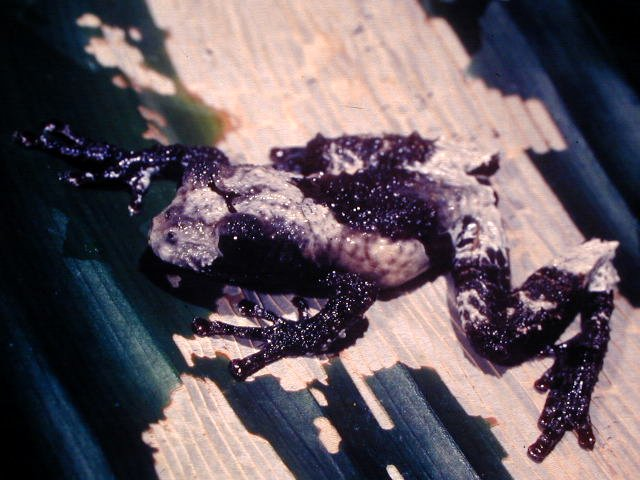
\includegraphics[width=.5\textwidth]{thelodermaasper.JPG}
\caption{In case you were wondering what {\it Theloderma asper}, the 
``bird-shit frog'', looks like. I snapped this one in North-east India ages 
ago}
\end{figure}

You can group regexes into meaningful blocks using parentheses. For 
example, let's try matching a string consisting of an academic's name, 
email address and research area or interest (no need to type this into 
any python file): 
  
\begin{lstlisting}
MyStr = 'Samraat Pawar, s.pawar@imperial.ac.uk, Systems biology and 
ecological theory'

# without groups
match = re.search(r"[\w\s]*,\s[\w\.@]*,\s[\w\s&]*",MyStr)

match.group()
'Samraat Pawar, s.pawar@imperial.ac.uk, Systems biology and ecological theory'

match.group(0)
'Samraat Pawar, s.pawar@imperial.ac.uk, Systems biology and ecological theory'

# now add groups using ( )
match = re.search(r"([\w\s]*),\s([\w\.@]*),\s([\w\s&]*)",MyStr)

match.group(0)
'Samraat Pawar, s.pawar@imperial.ac.uk, Systems biology and ecological theory'

match.group(1)
'Samraat Pawar'

match.group(2)
's.pawar@imperial.ac.uk'

match.group(3)
'Systems biology and ecological theory'
\end{lstlisting}

Have a look at {\tt re4.py} in your code repository for more on parsing 
email addresses using regexes.  

\subsection{Some RegExercises}

These exercises are not for submission as part of your coursework, but 
we will discuss them in class (in a later week).

\begin{enumerate}\itemsep16pt

	 \item Translate the following regular expressions into regular 
	 English (don't type this in {\tt regexs.py})!
  
\begin{lstlisting}
r'^abc[ab]+\s\t\d'
% 'abca \t1'

r'^\d{1,2}\/\d{1,2}\/\d{4}$'
% '11/12/2004'

r'\s*[a-zA-Z,\s]+\s*'
% ' aBz  '
\end{lstlisting}
  
\item Write a regex to match dates in format YYYYMMDD, making sure that:
     \begin{compactitem}
      \item Only seemingly valid dates match (i.e., year greater than 1900)
      \item First digit in month
 is either 0 or 1
      \item First digit in day $\leq$ 3
     \end{compactitem}
  
  \end{enumerate}
  
  %re.search(r'19\d{2}[01]\d[0-3]\d|20\d{2}[01]\d[0-3]\d', 'whatabout 19001212 ?').group()
  
  %Same, but shorter:
  % re.search(r'(19|20)\d{2}[01]\d[0-3]\d', 'whatabout 19001212?').group()

	% A more robust solution (Leanne Massie 2015-16 batch):

  % re.search(r'((19)|(20))\d{2}((0\d)|(10)|(11)|(12))([012]\d|((30)|(31)))' ,'whatabout 19001212 ?').group()
  % re.search(r'((19)|(20))\d{2}((0\d)|(10)|(11)|(12))([012]\d|((30)|(31)))' ,'whatabout 19001235 ?').group()  

\subsection{Important {\tt re} functions}

\begin{tabular}{p{5.4cm} p{9cm}} 
   
  {\tt re.compile(reg)} & Compile a regular expression. In this way
    the pattern is stored for repeated use, improving the speed.\\

	{\tt re.search(reg, text)} & Scan the string and find the first match 
	of the pattern in the string. Returns a {\tt match} object if 
	successful and {\tt None} otherwise.\\

	{\tt re.match(reg, text)} & as {\tt re.search}, but only match the 
	beginning of the string.\\

	{\tt re.split(ref, text)} & Split the text by the occurrence of the 
	pattern described by the regular expression.\\

	{\tt re.findall(ref, text)} & As {\tt re.search}, but return a list 
	of all the matches. If groups are present, return a list of groups.\\

	{\tt re.finditer(ref, text)} & As {\tt re.search}, but return an 
	iterator containing the next match.\\

	{\tt re.sub(ref, repl, text)} & Substitute each non-overlapping 
	occurrence of the match with the text in {\tt repl} (or a 
	function!).\\

\end{tabular}

\section{Practicals}
As always, test, add, commit and push all your new code and data to 
your git repository. 

\subsubsection{Blackbirds problem}

Complete the code {\tt blackbirds.py} that you find in the {\tt 
CMEEMasteRepo} (necessary data file is also there).

\section{Databases and {\tt python}}

Many of you will deal with complex data --- and often, lots of it. 
Ecological and Evolutionary data are particularly complex because they 
contain large numbers of attributes, often measured in very different 
scales and units for individual taxa, populations, etc. In this 
scenario, storing the data in a database makes a lot of sense! You can 
easily include the database in your analysis workflow --- indeed, 
that's why people use databases. And you can use python (and R) to 
build, manipulate and use your database.   

\subsection{Relational databases}

A {\it relational} database is a collection of interlinked ({\it 
related}) tables that altogether store a complex dataset in a logical, 
computer-readable format. Dividing a dataset into multiple tables 
minimizes redundancies. For example, if your data were sampled from 
three sites --- then, rather than repeating the site name and 
description in each row in a text file, you could just specify a 
numerical ``key'' that directs to another table containing the sampling 
site name and description.

Finally, if you have many rows in your data file, the type of 
sequential access we have been using in our {\tt python} and {\tt R} 
scripts is inefficient --- you should be able to instantly access any 
row regardless of its position

Data columns in a database are usually called {\it fields}, while the 
rows are the {\it records}. Here are a few things to keep in mind about 
databases:
 \begin{compactitem}
		\item Each field typically contains only one data type (e.g., 
			integers, floats, strings)
		\item Each record is a ``data point'', composed of different 
		values, one for each field --- somewhat like a python tuple
		\item Some fields are special, and are called {\it keys}:
      \begin{compactitem}
				\item The {\it primary key} uniquely defines a record in a 
				table (e.g., each row is identified by a unique number)
				\item To allow fast retrieval, some fields (and typically all the 
				keys) are indexed --- a copy of certain columns that can be searched 
				very efficiently 
				\item {\it Foreign keys} are keys in a table that are primary 
				keys in another table and define relationships between the 
				tables
      \end{compactitem}
		\item The key to designing a database is to minimize redundancy and 
		dependency without losing the logical consistency of tables --- 
		this is called {\it normalization} (arguably more of an art than a 
		science!)
\end{compactitem}

\noindent Let's look at a simple example. 

Imagine you recorded body 
sizes of species from different field sites in a single text file 
(e.g., a {\tt .csv} file) with the following fields:
  
\begin{tabular}{p{4cm} p{8cm}}
		{\tt ID} & Unique ID for the record\\
		{\tt SiteName} & Name of the site\\
	  {\tt SiteLong} & Longitude of the site\\
	  {\tt SiteLat} & Latitude of the site\\
	  {\tt SamplingDate} & Date of the sample\\
	  {\tt SamplingHour} & Hour of the sampling\\
	  {\tt SamplingAvgTemp} & Average air temperature on the sampling day\\
	  {\tt SamplingWaterTemp} & Temperature of the water\\
	  {\tt SamplingPH} & PH of the water\\
	  {\tt SpeciesCommonName} & Species of the sampled individual\\
	  {\tt SpeciesLatinBinom} & Latin binomial of the species\\
	  {\tt BodySize} & Width of the individual\\
	  {\tt BodyWeight} & Weight of the individual\\
\end{tabular}\\
  
It would be logical to divide the data into four tables:

{\it Site table}:\\
	\begin{tabular}{p{3cm} p{6cm}}
		{\tt SiteID} & ID for the site\\
		{\tt SiteName} & Name of the site\\
		{\tt SiteLong} & Longitude of the site\\
		{\tt SiteLat} & Latitude of the site\\
	\end{tabular}\\

{\it Sample table}:\\
	\begin{tabular}{p{4cm} p{6cm}}
		{\tt SamplingID} & ID for the sampling date\\
		{\tt SamplingDate} & Date of the sample\\
		{\tt SamplingHour} & Hour of the sample\\
		{\tt SamplingAvgTemp} & Average air temperature\\
		{\tt SamplingWaterTemp} & Temperature of the water\\
		{\tt SamplingPH} & PH of the water\\
	\end{tabular}\\
    
{\it Species table}:\\
	\begin{tabular}{p{4cm} p{6cm}}
     {\tt SpeciesID} & ID for the species\\
     {\tt SpeciesCommonName} & Species name\\
     {\tt SpeciesLatinBinom} & Latin binomial of the species\\
    \end{tabular}\\

  {\it Individual table}:\\
 	 \begin{tabular}{p{3cm} p{6cm}}
      {\tt IndividualID} & ID for the individual sampled\\
      {\tt SpeciesID} & ID for the species\\
      {\tt SamplingID} & ID for the sampling day\\
      {\tt SiteID} & ID for the site\\
      {\tt BodySize} & Width of the individual\\
      {\tt BodyWeight} & Weight of the individual\\
    \end{tabular}\\
 
In each table, the first ID field is the primary key. The last table 
contains three foreign keys because each individual is associated with 
one species, one sampling day and one sampling site. 

These structural features of a database are called its {\it schema}.

\subsection{SQLite}

{\tt SQLite} is a simple (and very popular) SQL (Structured Query 
Language)-based solution for managing localized, personal databases. I 
can safely bet that most, if not all of you unknowingly (or knowingly!) 
use {\tt SQLite}  --- it is used by MacOSX, Firefox, Acrobat Reader, 
iTunes, Skype, iPhone, etc. SQLite is also the database ``engine'' 
underlying your Siwlood Masters Web App: 
\url{http://silwoodmasters.co.uk}

We can easily use SQLite through Python scripts. First, install 
SQLite by typing in the Ubuntu terminal:
\begin{lstlisting}
$ sudo apt-get install sqlite3 libsqlite3-dev
\end{lstlisting}

Also, make sure that you have the necessary package for python by 
typing {\tt import sqlite3} in the python or ipython shell. Finally, 
you may install a GUI for SQLite3 :

\begin{lstlisting}
$ sudo apt-get install sqliteman
\end{lstlisting}

Now type {\tt sqlite3} in the Ubuntu terminal to check if SQLite 
successfully launches. 

SQLite has very few data types (and lacks a boolean and a date type):

\begin{tabular}{p{2cm} p{10cm}} 
	{\tt NULL} & The value is a NULL value\\
  {\tt INTEGER} & The value is a signed integer, stored in up to or 8
	bytes\\
  {\tt REAL} & The value is a floating point value, stored as in 8 
  bytes\\
  {\tt TEXT} & The value is a text string\\
  {\tt BLOB} & The value is a blob of data, stored exactly as it was
	input (useful for binary types, such as bitmap images or pdfs)\\
\end{tabular}\\

Typically, you will build a database by importing csv data --- be aware 
that:
    \begin{compactitem}
      \item Headers: the csv should have no headers
			\item Separators: if the comma is the separator, each record 
			should not contain any other commas
      \item Quotes: there should be no quotes in the data
      \item Newlines: there should be no newlines
    \end{compactitem}

		Now build your first database in SQLite! We will use as example a 
		global dataset on metabolic traits called {\it Biotraits} that we 
		are currently developing in our lab (should be in your {\tt Data} 
		directory). This dataset contains 164 columns (fields). Thermal 
		response curves for different traits and species are stored in 
		rows. This means that site description or taxonomy  are repeated as 
		many times as temperatures are measured in the curve. You can 
		imagine how much redundacy can be here!!!

		For this reason, it is easier to migrate the dataset to SQL and 
		split it into several tables:
    
    \begin{compactitem}
    \item TCP: Includes the thermal curve performance for each species and trait (as many rows per trait and species
      as temperatures have been measured within the TCP)
    \item TraitInfo: Contains site description and conditions under the traits were measured (one row per thermal curve)
    \item Consumer: Consumer description including taxonomy (one row per thermal curve).
    \item Resource: Resource description including taxonomy (one row per thermal curve).
    \item Size: Size data for each species (one row per thermal curve)
    \item DataSource: Contains information about the data source (citation, contributors) (one row per thermal curve).
    \end{compactitem}

    So all these tables compose the {\it Biotraits} {\tt schema}.

    Navigate to your {\tt Data} directory and in an Ubuntu terminal type:

\begin{lstlisting}
$ sqlite3 Biotraits.db
SQLite version 3.7.9
Enter ".help" for instructions
Enter SQL statements terminated with a ";"
\end{lstlisting}
This creates an empty database in your {\tt Data} directory. Now, you 
need to create a table with some fields. Let's start with the {\it TraitInfo} table:
\begin{lstlisting}
	
sqlite> CREATE TABLE TraitInfo (Numbers integer primary key,
   ...>                                 OriginalID text,
   ...>                                 FinalID text,
   ...>                                 OriginalTraitName text,
   ...>                                 OriginalTraitDef text,
   ...>                                 Replicates integer,
   ...>                                 Habitat  integer,               
   ...>                                 Climate text,
   ...>                                 Location text,
   ...>                                 LocationType text,
   ...>                                 LocationDate text,
   ...>                                 CoordinateType text,
   ...>                                 Latitude integer,
   ...>                                 Longitude integer);

\end{lstlisting}

Note that I am writing all SQL commands in upper case, but it is not 
necessary. I am using upper case here because SQL syntax is long and 
clunky, and it quickly becomes hard to spot (and edit) commands in long 
strings of complex queries.     

Now let's import the dataset:

\begin{lstlisting}
sqlite> .mode csv

sqlite> .import TraitInfo.csv TraitInfo
\end{lstlisting}

So we built a table and imported a csv file into it. Now we can ask 
SQLite to show all the tables we currently have:

% \item The general procedure is:
% \begin{lstlisting}
% sqlite> create table test (id integer, name type, ...);
% 
% sqlite> .separator ","
% 
% sqlite> .import no_yes.csv test
  % \end{lstlisting}

\begin{lstlisting}
sqlite> .tables

TraitInfo
\end{lstlisting}

Let's run our first {\it Query} (note that you need a semicolon to end 
a command):

\begin{lstlisting}
sqlite> SELECT * FROM TraitInfo LIMIT 5;

1,1,MTD1,"Resource Consumption Rate","The number of resource consumed per number of consumers per time",6,freshwater,temperate,"Eunice Lake; Ontario; Canada",NA,NA,NA,51.254,-85.323
2,1,MTD1,"Resource Consumption Rate","The number of resource consumed per number of consumers per time",6,freshwater,temperate,"Eunice Lake; Ontario; Canada",NA,NA,NA,51.254,-85.323
3,1,MTD1,"Resource Consumption Rate","The number of resource consumed per number of consumers per time",6,freshwater,temperate,"Eunice Lake; Ontario; Canada",NA,NA,NA,51.254,-85.323
4,2,MTD2,"Resource Consumption Rate","The number of resource consumed per number of consumers per time",6,freshwater,temperate,"Eunice Lake; Ontario; Canada",NA,NA,NA,51.254,-85.323
5,2,MTD2,"Resource Consumption Rate","The number of resource consumed per number of consumers per time",6,freshwater,temperate,"Eunice Lake; Ontario; Canada",NA,NA,NA,51.254,-85.323

\end{lstlisting}
  
Let's turn on some nicer formatting:

\begin{lstlisting}
sqlite> .mode column

sqlite> .header ON

sqlite> SELECT * FROM TraitInfo LIMIT 5;

Numbers  OriginalID  FinalID     OriginalTraitName           ... 
-------  ----------  ----------  -------------------------   ...
1        1           MTD1        Resource Consumption Rate   ...
4        2           MTD2        Resource Consumption Rate   ...
6        3           MTD3        Resource Consumption Rate   ...
9        4           MTD4        Resource Mass Consumption   ...
12       5           MTD5        Resource Mass Consumption   ...

\end{lstlisting}
  
The main statement to select records from a table is {\tt SELECT}:
 
\begin{lstlisting}
sqlite> .width 40  ## NOTE: Control the width

sqlite> SELECT DISTINCT OriginalTraitName FROM TraitInfo; # Returns unique values

OriginalTraitName                       
----------------------------------------
Resource Consumption Rate               
Resource Mass Consumption Rate          
Mass-Specific Mass Consumption Rate     
Voluntary Body Velocity                 
Forward Attack Distance                 
Foraging Velocity                       
Resource Reaction Distance                   
....

sqlite> SELECT DISTINCT Habitat FROM TraitInfo
   ...> WHERE OriginalTraitName = "Resource Consumption Rate"; # Sets a condition

Habitat                                 
----------------------------------------
freshwater                              
marine                                  
terrestrial 

sqlite> SELECT COUNT (*) FROM TraitInfo;  # Returns number of rows

Count (*)           
--------------------
2336

sqlite> SELECT Habitat, COUNT(OriginalTraitName) # Returns number of rows for each group
   ...> FROM TraitInfo GROUP BY Habitat;

Habitat     COUNT(OriginalTraitName)
----------  ------------------------
NA          16                      
freshwater  609                     
marine      909                     
terrestria  802   

sqlite> SELECT COUNT(DISTINCT OriginalTraitName) # Returns number of unique values
   ...> FROM TraitInfo;

COUNT(DISTINCT OriginalTraitName)
---------------------------------
220   

sqlite> SELECT COUNT(DISTINCT OriginalTraitName) TraitCount # Assigns alias to the variable
   ...> FROM TraitInfo;

TraitCount
----------
220 

sqlite> SELECT Habitat,
   ...> COUNT(DISTINCT OriginalTraitName) AS TN
   ...> FROM TraitInfo GROUP BY Habitat;

Habitat     TN        
----------  ----------
NA          7         
freshwater  82        
marine      95        
terrestria  96     


sqlite> SELECT * # WHAT TO SELECT
   ...> FROM TraitInfo # FROM WHERE
   ...> WHERE Habitat = "marine" # CONDITIONS
   ...> AND OriginalTraitName = "Resource Consumption Rate";

Numbers     OriginalID  FinalID     OriginalTraitName          ...
----------  ----------  ----------  -------------------------  ...
778         308         MTD99       Resource Consumption Rate  ...
798         310         MTD101      Resource Consumption Rate  ...
806         311         MTD102      Resource Consumption Rate  ...
993         351         MTD113      Resource Consumption Rate  ...

\end{lstlisting}

The structure of the {\tt SELECT} commend is as follows ({\it Note: 
{\bf all} characters are case {\bf in}sensitive}):
\begin{verbatim}
	SELECT [DISTINCT] field
	FROM table
	WHERE predicate
	GROUP BY field
	HAVING predicate
	ORDER BY field
	LIMIT number
	;
\end{verbatim}

Let's try some more elaborate queries:

\begin{lstlisting} 
sqlite> SELECT Numbers FROM TraitInfo LIMIT 5;

Numbers   
----------
1         
4         
6         
9         
12      

sqlite> SELECT Numbers 
   ...> FROM TraitInfo
   ...> WHERE Numbers > 100 
   ...> AND Numbers < 200;

Numbers   
----------
107       
110       
112       
115         

sqlite> SELECT Numbers 
   ...> FROM TraitInfo
   ...> WHERE Habitat = "freshwater"
   ...> AND Number > 700
   ...> AND Number < 800;

Numbers   
----------
704       
708       
712       
716       
720       
725       
730       
735       
740       
744       
748       
      
\end{lstlisting}

You can also match records using something like regular expressions. In 
SQL, when we use the command {\tt LIKE}, the percent \% symbol matches 
any sequence of zero or more characters and the underscore matches any 
single character. Similarly, {\tt GLOB} uses the asterisk and the 
underscore.

 \begin{lstlisting} 
sqlite> SELECT DISTINCT OriginalTraitName
   ...> FROM TraitInfo
   ...> WHERE OriginalTraitName LIKE "_esource Consumption Rate";

OriginalTraitName        
-------------------------
Resource Consumption Rate          

sqlite> SELECT DISTINCT OriginalTraitName
   ...> FROM TraitInfo
   ...> WHERE OriginalTraitName LIKE "Resource%";

OriginalTraitName                       
----------------------------------------
Resource Consumption Rate               
Resource Mass Consumption Rate          
Resource Reaction Distance              
Resource Habitat Encounter Rate         
Resource Consumption Probability        
Resource Mobility Selection             
Resource Size Selection                 
Resource Size Capture Intent Acceptance 
Resource Encounter Rate                 
Resource Escape Response Probability 

sqlite> SELECT DISTINCT OriginalTraitName
   ...> FROM TraitInfo
   ...> WHERE OriginalTraitName GLOB "Resource*";


OriginalTraitName                       
----------------------------------------
Resource Consumption Rate               
Resource Mass Consumption Rate          
Resource Reaction Distance              
Resource Habitat Encounter Rate         
Resource Consumption Probability        
Resource Mobility Selection             
Resource Size Selection                 
Resource Size Capture Intent Acceptance 
Resource Encounter Rate                 
Resource Escape Response Probability 

# NOTE THAT GLOB IS CASE SENSITIVE, WHILE LIKE IS NOT

sqlite> SELECT DISTINCT OriginalTraitName
   ...> FROM TraitInfo
   ...> WHERE OriginalTraitName LIKE "resource%";

OriginalTraitName                       
----------------------------------------
Resource Consumption Rate               
Resource Mass Consumption Rate          
Resource Reaction Distance              
Resource Habitat Encounter Rate         
Resource Consumption Probability        
Resource Mobility Selection             
Resource Size Selection                 
Resource Size Capture Intent Acceptance 
Resource Encounter Rate                 
Resource Escape Response Probability 

\end{lstlisting}

We can also order by any column:

 \begin{lstlisting}
sqlite> SELECT OriginalTraitName, Habitat FROM 
   ...>  TraitInfo LIMIT 5;

OriginalTraitName          Habitat   
-------------------------  ----------
Resource Consumption Rate  freshwater
Resource Consumption Rate  freshwater
Resource Consumption Rate  freshwater
Resource Mass Consumption  freshwater
Resource Mass Consumption  freshwater

sqlite> SELECT OriginalTraitName, Habitat FROM 
   ...> TraitInfo ORDER BY OriginalTraitName LIMIT 5;

OriginalTraitName           Habitat   
--------------------------  ----------
48-hr Hatching Probability  marine    
Asexual Reproduction Rate   marine    
Attack Body Acceleration    marine    
Attack Body Velocity        marine    
Attack Body Velocity        marine  
 \end{lstlisting}


 Until now we have just queried data from one single table, but as we have seen,
 the point of storing a database in SQL is that we can use multiple tables minimizing
 redundancies within them. And of course, querying data from those different tables at
 the same time will be necessary at some point.

 Let's import then one more table to our database:

 \begin{lstlisting}
 sqlite> CREATE TABLE Consumer (Numbers integer primary key,
   ...>                                OriginalID text,
   ...>                                FinalID text,
   ...>                                Consumer text,
   ...>                                ConCommon text,
   ...>                                ConKingdom text,
   ...>                                ConPhylum text,
   ...>                                ConClass text,
   ...>                                ConOrder text,
   ...>                                ConFamily text,
   ...>                                ConGenus text,
   ...>                                ConSpecies text);

 
sqlite> .import Consumer.csv Consumer

# Now we have two tables in our database:

sqlite> .tables
Consumer   TraitInfo

 
# These tables are connected by two differents keys: OriginalID
# and FinalID. These are unique IDs for each thermal curve. For each
# FinalID we can get the trait name (OriginalTraitName) from the TraitInfo
# table and the corresponding species name (ConSpecies) from the Consumer table.

sqlite> SELECT A1.FinalID, A1.Consumer, A2.FinalID,  A2.OriginalTraitName
   ...> FROM Consumer A1, TraitInfo A2
   ...> WHERE A1.FinalID=A2.FinalID LIMIT 8;

FinalID     Consumer               FinalID     OriginalTraitName        
----------  ---------------------  ----------  -------------------------
MTD1        Chaoborus trivittatus  MTD1        Resource Consumption Rate
MTD2        Chaoborus trivittatus  MTD2        Resource Consumption Rate
MTD3        Chaoborus americanus   MTD3        Resource Consumption Rate
MTD4        Stizostedion vitreum   MTD4        Resource Mass Consumption
MTD5        Macrobrachium rosenbe  MTD5        Resource Mass Consumption
MTD6        Ranatra dispar         MTD6        Resource Consumption Rate
MTD7        Ceriodaphnia reticula  MTD7        Mass-Specific Mass Consum
MTD8        Polyphemus pediculus   MTD8        Voluntary Body Velocity 

# In the same way we assign alias to variables, we can use them for tables.

\end{lstlisting}
 This example seems easy because both tables have the same number of rows. But the
 query is still as simple when we have tables with different rows.

\begin{lstlisting}
# Let's import the TCP table:

sqlite> CREATE TABLE TCP (Numbers integer primary key,
   ...>                           OriginalID text,
   ...>                           FinalID text,
   ...>                           OriginalTraitValue integer,
   ...>                           OriginalTraitUnit text,
   ...>                           LabGrowthTemp integer,
   ...>                           LabGrowthTempUnit text,   
   ...>                           ConTemp integer,
   ...>                           ConTempUnit text,
   ...>                           ConTempMethod text,
   ...>                           ConAcc text,
   ...>                           ConAccTemp integer);


sqlite> .import TCP.csv TCP
sqlite> .tables
Consumer   TCP        TraitInfo
                          
# Now imagine we want to query the thermal performance curves that we have
# stored for the species Mytilus edulis. Using the FinalID to match the tables,
# the query can be as simple as:

sqlite> SELECT A1.ConTemp, A1.OriginalTraitValue, A2.OriginalTraitName, A3.Consumer
   ...> FROM TCP A1, TraitInfo A2, Consumer A3
   ...> WHERE A1.FinalID=A2.FinalID AND A3.ConSpecies="Mytilus edulis" AND A3.FinalID=A2.FinalID LIMIT 8

ConTemp     OriginalTraitValue    OriginalTraitName               Consumer            
----------  --------------------  ------------------------------  --------------------
25          2.707075              Filtration Rate                 Mytilus edulis      
20          3.40721               Filtration Rate                 Mytilus edulis      
5           3.419455              Filtration Rate                 Mytilus edulis      
15          3.711165              Filtration Rate                 Mytilus edulis      
10          3.875465              Filtration Rate                 Mytilus edulis      
5           0.34                  In Vitro Gill Particle Transpo  Mytilus edulis      
10          0.46                  In Vitro Gill Particle Transpo  Mytilus edulis      
15          0.595                 In Vitro Gill Particle Transpo  Mytilus edulis

 \end{lstlisting}                          

So on and so forth (joining tables etc. would come next...). But if you 
want to keep practicing and learn more about sqlite commands, this is a 
very useful site: \url{http://www.sqlite.org/sessions/sqlite.html}. You 
can store your queries and database management commands in an {\tt 
.sql} file ({\tt geany} will take care of syntax highlighting etc.)

\subsection{SQLite with python}   
It is easy to access, update and manage SQLite databases with {\tt 
python} (you should have this script file in your {\tt Code} 
directory):
 
\lstinputlisting{Practicals/Code/pythonsql.py}
 
You can create a database in memory, without using the disk --- thus 
you can create and discard an SQLite database within your workflow!:

\lstinputlisting{Practicals/Code/sqlitemem.py}

\section{Using {\tt python} to build workflows}

You can use python to build an automated data analysis or simulation 
workflow that involves multiple applications, especially the ones you 
have already learnt: {\tt R}, \LaTeX, \& UNIX {\tt bash}. For example, 
you could, in theory, write a single Python script to generate and 
update your masters dissertation, tables, plots, and all. Python is 
ideal for building such workflows because it has packages for 
practically every purpose (see Section on Packages above).

\subsection{Using {\tt subprocess}}

The {\tt subprocess} module is particularly important as it can run 
other applications, including R. Let's try -- first launch {\tt 
ipython}, then {\tt cd} to your python code directory, and type:
\begin{lstlisting}
import subprocess
subprocess.os.system("geany boilerplate.py")
subprocess.os.system("gedit ../Data/TestOaksData.csv")
subprocess.os.system("python boilerplate.py") # A bit silly! 
\end{lstlisting}
  
Easy as pie! You will notice that the terminal remains ``connected'' to 
geany after you run the first of the three lines above, and you have 
to quit geany to go on to launcing gedit. To avoid this, you can do:    

\begin{lstlisting}
subprocess.os.system("geany boilerplate.py &")
subprocess.os.system("gedit ../Data/TestOaksData.csv &")
subprocess.os.system("python boilerplate.py &") # A bit silly! 
\end{lstlisting}

Adding a {\tt \&} after a program call, i.e., {\tt geany boilerplate.py 
\&} instead of {\tt geany boilerplate.py} disconnects the terminal and 
allows you to run sequential commands in the terminal/bash.
 
Similarly, to compile your \LaTeX document (using {\tt pdflatex} in this case):

\begin{lstlisting}
subprocess.os.system("pdflatex yourlatexdoc.tex")
\end{lstlisting}
  
You can also do this (instead of using {\tt subprocess.os}):
\begin{lstlisting}
subprocess.Popen("geany boilerplate.py", shell=True).wait()
\end{lstlisting}
  
You can also use {\tt subprocess.os} to make your code OS (Linux, 
Windows, Mac) independent. For example to assign paths:
\begin{lstlisting}
subprocess.os.path.join('directory', 'subdirectory', 'file')
\end{lstlisting}

The result would be appropriately different on Windows (with 
backslashes instead of forward slashes). 

Note that in all cases you can "catch" the output of {\tt subprocess} 
so that you can then use the output within your python script. A simple
example, where the output is a platform-dependent directory path, is: 
\begin{lstlisting}
MyPath = subprocess.os.path.join('directory', 'subdirectory', 'file')
\end{lstlisting}
Explore what {\tt subprocess} can do by tabbing {\tt subprocess.}, and 
also for submodules, e.g., type {\tt subprocess.os.} and then tab.

\subsection{Running {\tt R}}

R is likely an important part of your project's analysis and data 
visualization components in particular --- for example for  statistical 
analyses and pretty plotting (Ahem. {\tt ggplot2}). 

You can run {\tt R} from Python pretty easily. Try the following:

\begin{compactitem}[$\quad\star$]

\item Create an R script file called {\tt TestR.R} in your {\tt 
Week6/Code} with the following content:
\begin{lstlisting}
print("Hello, this is R!")
\end{lstlisting}

\item Now, create {\tt TestR.py} in {\tt CMEECourseWork/Week6/Code} with the 
following content :
\begin{lstlisting}
import subprocess
subprocess.Popen("/usr/lib/R/bin/Rscript --verbose TestR.R > \
../Results/TestR.Rout 2> ../Results/TestR_errFile.Rout",\
 shell=True).wait()
\end{lstlisting}

{\it Note the backslashes} --- this is so that {\tt python} can read 
the mutiline script as a single line.

\item Now run {\tt TestR.py} (or {\tt \%cpaste}) and check {\tt TestR.Rout} 
and {\tt TestR\_errorFile.Rout}. 

\item Also check what happens if you run (type directly in {\tt 
ipython} or {\tt python} console):
\begin{lstlisting}
subprocess.Popen("/usr/lib/R/bin/Rscript --verbose NonExistScript.R > \
../Results/outputFile.Rout 2> ../Results/errorFile.Rout", \
shell=True).wait()
\end{lstlisting}

\end{compactitem}

\begin{tipbox}
It is possible that the location of {\tt RScript} is different in your 
Ubuntu install. To locate it, try {\tt find /usr -name 'Rscript'} in the linux
terminal (not in {\tt python}!).
\end{tipbox}

What do you see on the screen? Now check {\tt outputFile.Rout} and 
{\tt errorFile.Rout}.

\section{Practicals}
As always, test, add, commit and push all your new code and data to 
your git repository. 
	
\subsubsection{Using {\tt os} problem 1} 
	
	Open {\tt using\_os.py} and complete the tasks assigned \\
	(hint: you might want to look at {\tt subprocess.os.walk()})
	
\subsubsection{Using {\tt os} problem 2}
	
	 Open {\tt fmr.R} and work out what it does; check that you have 
	{\tt NagyEtAl1999.csv}. Now write python code called 
		{\tt run\_fmr\_R.py} that:
	\begin{compactitem} \itemsep2pt
		\item Runs {\tt fmr.R} to generate the desired result
		\item {\tt run\_fmr\_R.py} should also print to the python screen 
		whether the run was successful, and the contents of the R console 
		output
	\end{compactitem}

\section{Practicals wrap-up}

  \begin{enumerate}

	\item Review and make sure you can run all the commands, code 
	fragments, and scripts we have till now and get the expected outputs 
	---  all scripts should work on any other linux laptop.
	
	\item Include an appropriate docstring (if one is missing) at the 
	beginning of {\it each} of each of the python script / module files 
	you have written, as well as at the start of every function (or 
	sub-module) in a module.

	\item Also annotate your code lines as much and as often as necessary 
	using \#.
	
	\item Keep all files organized in {\tt CMEECourseWork}.
	
	\item {\tt git add}, {\tt commit} and {\tt push} all your week's  code 
	and data to your git repository by next Wednesday. 
	 
   \end{enumerate}
	
\section{Readings and Resources}

\begin{compactitem} \itemsep6pt
	\item \url{http://matplotlib.org/}
	\item For SciPy, the official documentation is great:\\
\url{https://docs.scipy.org/doc/scipy/reference/}\\
	Read about the scipy modules you think will be important to you. 
	
	\item The ``ecosystem'' for Scientific computing in python: 
	\url{http://www.scipy-lectures.org/}

	\item A Primer on Scientific Programming with Python 
	\url{http://www.springer.com/us/book/9783642549595}; 
	Multiple copies of this book are available from the central library 
	and can be requested to Silwood from the IC library website. 
	You can also find a pdf - google it

	\item Many great examples of applications in the scipy cookbook:
	\url{https://lagunita.stanford.edu/courses/DB/2014/SelfPaced/about}

	\item \url{https://docs.python.org/2/howto/regex.html}
	\item Google's short class on regex in python:\\
	\url{https://developers.google.com/edu/python/regular-expressions}
	\item \url{http://www.regular-expressions.info/} has a good intro, tips and 
	a great array of canned solutions
	\item Use and abuse of regex:\\ 
\url{https://blog.codinghorror.com/regex-use-vs-regex-abuse/}   


	\item ``The Definitive Guide to SQLite'' is a pretty complete guide 
	to SQLite and freely available from \url{ 
	http://sd.blackball.lv/library/The_Definitive_Guide_to_SQLite_2nd_edition.pdf}
	\item For databses in general, try the Stanford Introduction to 
	Databases course: \url{https://www.coursera.org/course/db} 

\end{compactitem}
